\documentclass[11pt]{article}
\usepackage{amsmath,amsbsy,amssymb,verbatim,fullpage,ifthen,graphicx,bm,amsfonts,amsthm}
\usepackage{graphicx}
\usepackage{xcolor}
\newcommand{\mfile}[1]  {{\small \verbatiminput{./#1}}} % Jeff Fessler, input matlab file
\newcommand{\tmop}[1]{\ensuremath{\operatorname{#1}}}

\newcommand{\R}{\mathbb{R}}
\newcommand{\C}{\mathbb{C}}
\newcommand{\Z}{\mathbb{Z}}
\newcommand{\A}{\mathcal{A}}
\newcommand{\minimize}{\operatorname*{minimize\ }}
\newcommand{\maximize}{\operatorname*{maximize}}

%\newcommand{\mfile}[1]  {{\small \verbatiminput{./#1}}} 
$ \newcommand{\mtx}[1]{\mathbf{#1}}
\newcommand{\vct}[1]{\mathbf{#1}}
\def \lg       {\langle}
\def \rg       {\rangle}
\def \mA {\mtx{A}}
\def \mI {\mtx{I}}
\def \mU {\mtx{U}}
\def \mS {\mtx{S}}
\def \mV {\mtx{V}}
\def \mW {\mtx{W}}
\def \mLambda {\mtx{\Lambda}}
\def \mX {\mtx{X}}
\def \mY {\mtx{Y}}
\def \mZ {\mtx{Z}}
\def \zero     {\mathbf{0}}
\def \vzero    {\vct{0}}
\def \vone    {\vct{1}}
\def \vu {\vct{u}}
\def \vv {\vct{v}}
\def \vx {\vct{x}}
\def \vy {\vct{y}}
\def \vz {\vct{z}}
\def \vphi {\vct{\phi}}
\def \vmu {\vct{\mu}}
\def \R {\mathbb{R}} $


\usepackage{xspace}

\makeatletter
\DeclareRobustCommand\onedot{\futurelet\@let@token\@onedot}
\def\@onedot{\ifx\@let@token.\else.\null\fi\xspace}

\def\eg{\emph{e.g}\onedot} \def\Eg{\emph{E.g}\onedot}
\def\ie{\emph{i.e}\onedot} \def\Ie{\emph{I.e}\onedot}
\def\cf{\emph{c.f}\onedot} \def\Cf{\emph{C.f}\onedot}
\def\etc{\emph{etc}\onedot} \def\vs{\emph{vs}\onedot}
\def\wrt{w.r.t\onedot} \def\dof{d.o.f\onedot}
\def\etal{\emph{et al}\onedot} \def\st{\emph{s.t}\onedot}
\pagestyle{plain}

\title{{\bf Homework Set 1, CPSC 8420, Spring 2022}}
\author{\Large\underline{LastName, FirstName}}
\date{\textbf{\Large\textcolor{red}{Due 03/03/2022, Thursday, 11:59PM EST}}}

\begin{document}
\maketitle

\section*{Ridge Regression}
Please show that for arbitrary $\mA\in\R^{n\times p}$, $(\mA^T\mA+\lambda\mI_p)^{-1}\mA^T=\mA^T(\mA\mA^T+\lambda\mI_n)^{-1}$, where $\lambda>0$. Now assume $n=100$, please compare the time consumption when $p=[10,100,1000,2000]$ and plot the results appropriately (\eg in one figure where $X$-axis denotes $p$ while $Y$-axis the time consumption).
%For PCA, from the perspective of minimizing reconstruction error, please derive the solution to $\minimize \limits_{\bm{\mu},\{\vv_i\},\mU_q} \sum_{i=1}^{N}\|\mX_i-\bm{\mu}-\mU_q \vv_i\|^2_2, \st \ \mU_q^T\mU_q=\mI_q$, where $\mX\in\R^{p\times N}, \bm{\mu}\in\R^p, \mU \in\R^{p\times q}, \vv_i \in \R^q$. 
\vspace{4cm}

\section*{Bias–variance trade-off for $k$-NN}
Assume $y=f(x)+\epsilon$ where $E(\epsilon)=0, Var(\epsilon)=\sigma^2$. Please show that:
\begin{equation}
	Err(x_0)=\sigma^2+\frac{\sigma^2}{k}+[f(x_0)-\frac{1}{k}\sum_{l=1}^{k}f(x_l)]^2,
\end{equation}
where $x_l$ denotes the nearest neighbour data.  Please justify Bias and Variance change when $k$ increases and explain if necessary.
%For PCA, from the perspective of maximizing variance, please show that the sotution of $\bm{\phi}$ to $\maximize \|\mX \bm{\phi}\|^2_2, \st \ \|\bm{\phi}\|_2=1$ is exactly the first column of $\mU$, where $[\mU,\mS,\mU]=svd(\mX^T\mX)$. (Note: you need prove why it is optimal than any other reasonable combinations of $\mU_i$, say $\hat{\bm{\phi}}=0.8*\mU(:,1)+0.6*\mU(:,2)$ which also  satisfies $\|\hat{\bm{\phi}}\|_2=1$.)
\vspace{4cm}

\section*{Shrinkage Methods}
For vanilla linear regression model: $\min \|\vy-\mA\bm{\beta}\|_2^2$, 
%where we set $\mA^T\mA=\mI$ for convinience, \frac{\lambda}{2}
we denote the solution as $\hat{\bm{\beta}}_{LS}$; for ridge regression model: $\min \|\vy-\mA\bm{\beta}\|_2^2+\lambda*\|\bm{\beta}\|_2^2$, we denote the solution as $\hat{\bm{\beta}}_\lambda^{Ridge}$; for Lasso model: $\min \frac{1}{2}\|\vy-\mA\bm{\beta}\|_2^2+\lambda*\|\bm{\beta}\|_1$, we denote the solution as $\hat{\bm{\beta}}_\lambda^{Lasso}$; for Subset Selection model:  $\min \frac{1}{2}\|\vy-\mA\bm{\beta}\|_2^2+\lambda*\|\bm{\beta}\|_0$, we denote the solution as $\hat{\bm{\beta}}_\lambda^{Subset}$, now please derive each $\hat{\bm{\beta}}$ given $\vy, \mA  (\st \ \mA^T\mA=\mI), \lambda$. Also, show the relationship of (each element in) $\hat{\bm{\beta}}_\lambda^{Ridge}, \hat{\bm{\beta}}_\lambda^{Lasso}, \hat{\bm{\beta}}_\lambda^{Subset}$ with (that in) $\hat{\bm{\beta}}_{LS}$ respectively. (you are encouraged to illustrate the relationship with figures appropriately.)
\vspace{4cm}

\section*{Linear Regression and its extension}
\begin{figure}
	\centering
	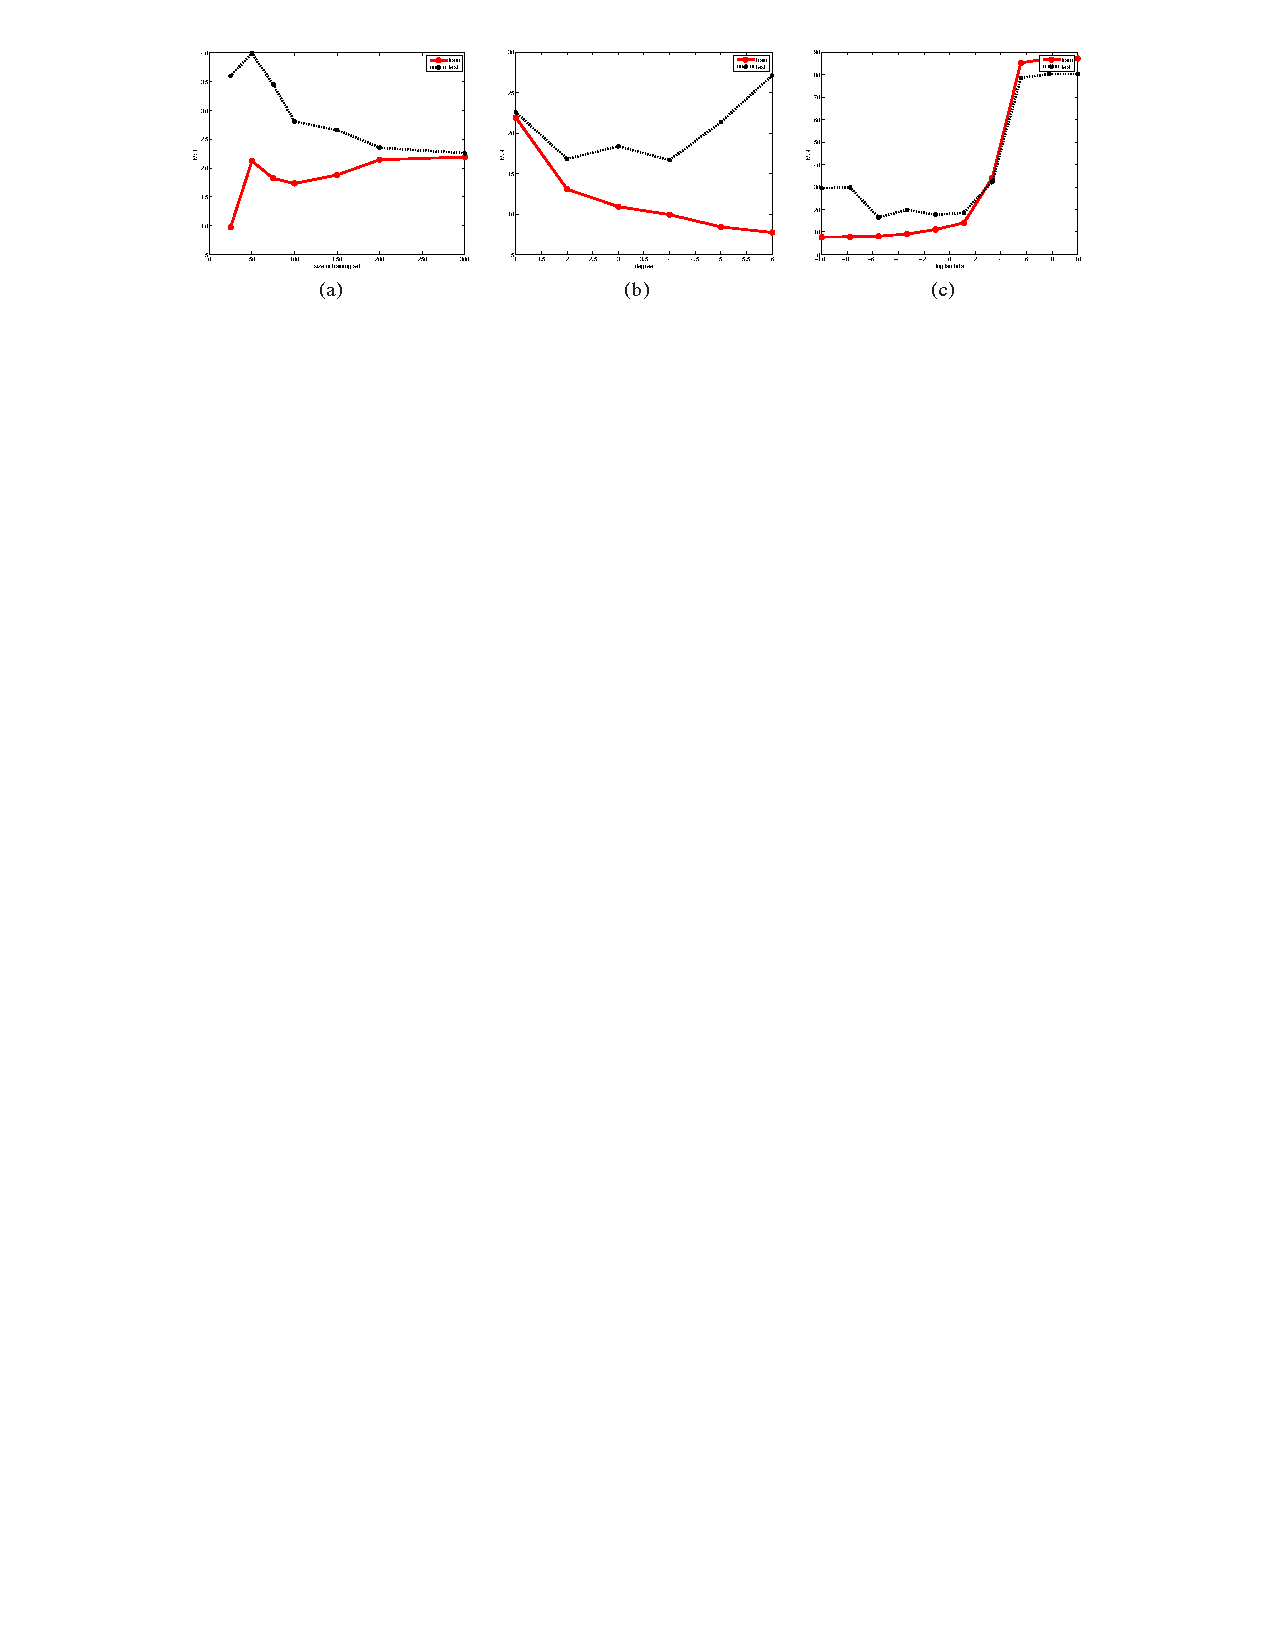
\includegraphics[width=1\linewidth]{fig}
	\caption{MSE vs (a) training set size, (b) polynomial degree, (c) size of ridge penalty. Solid Red = training, dotted black = test.}
	\label{fig:fig}
\end{figure}

In the Boston housing dataset, there are 506 records. We will
use first 13 features as inputs, $x$, and the 14th feature, median house price, as the output $y$. All features are continuous,
except feature 4, which is binary. However, we will treat this like any other continuous variable.
\begin{enumerate}
	\item Load the housing.data file. We will use the first 300 cases for training and the remaining 206 cases for
	testing. However, the records seem to be sorted in some kind of order. To eliminate this, we will shuffle the data
	before splitting into a training/test set. So we can all compare results, let use the following convention:
	\mfile{sample.m}
	\item Now extract the first n records of the training data, for $n \in \{25, 50, 75, 100, 150, 200, 300\}$. For each such
	training subset, standardize it (you may use \textit{zscore} function in Matlab), and fit a linear regression model using least squares. (Remember to include
	an offset term.) Then standardize the whole test set in the same way. Compute the mean squared error on
	the training subset and on the whole test set. Plot MSE versus training set size. You should get a plot like
	Figure 1(a). Turn in your plot and code. Explain why the test error decreases as n increases, and why the train
	error increases as n increases. Why do the curves eventually meet?
	As a debugging aid, here are the regression weights I get when I train on the first 25 cases (the first term is the
	offset, w0): $[26.11, -0.58, 3.02,\dots,-0.21, -0.27, -1.16]$.
	\item We will now replace the original features with an expanded set of features based on higher order terms. (We
	will ignore interaction terms.) For example, a quadratic expansion gives:
	\begin{equation}
		\begin{pmatrix}
			x_{11} & x_{12} & \dots & x_{1d} \\
			\vdots& \vdots & \ddots & \vdots \\
			x_{n1}& x_{n2} & \dots & x_{nd} \\
		\end{pmatrix}\xrightarrow[]{}\begin{pmatrix}
			x_{11} & x_{12} & \dots & x_{1d}& x_{11}^2 & x_{12}^2 & \dots & x_{1d}^2\\
			\vdots& \vdots & \ddots & \vdots&\vdots& \vdots & \ddots & \vdots \\
			x_{n1}& x_{n2} & \dots & x_{nd}& x_{n1}^2& x_{n2}^2 & \dots & x_{nd}^2\\
		\end{pmatrix}
	\end{equation}
The provided function degexpand(X,deg,addOnes) will replace each row of X with all powers up to degree deg. Use
this function to train (by least squares) models with degrees 1 to 6. Use all the the training data. Plot the MSE on
the training and test sets vs degree. You should get a plot like Figure 1(b). Turn in your plot and code. Explain
why the test error decreases and then increases with degree, and why the train error decreases with degree.
\item Now we will use ridge regression to regularize the degree 6 polynomial. Fit models using ridge regression with
the following values for $\lambda$:
$$lambdas=[0 \  logspace(-10,10,10)]$$
Use all the training data. Plot the MSE on the training and test sets vs $log_{10}(\lambda)$. You should get a plot like
Figure 1(c). Turn in your plot and code. Explain why the test error goes down and then up with increasing $\lambda$,
and why the train error goes up with increasing $\lambda$.
\item We turn to Lasso method with objective $\frac{1}{2}\|\mX \beta-y\|^2+\lambda\|\beta\|_1$ where $\lambda$ varies in: $$lambdas=[logspace(-10,10,10)]$$ and we make use of all training samples with no feature expansion. Please plot the changes of $\beta$ with $\lambda$ changes.
\end{enumerate}

%Why might we prefer to minimize the sum of absolute residuals instead of the residual sum of squares for some data sets? Recall clustering method $K$-means when calculating the controid, it is to take the mean value of the datapoints belonging to the same cluster, so what about $K$-medians? What is its advantage over of $K$-means? Please use a synthetic (toy) experiment to illustrate your conclusion.
% \vspace{4cm}
%\section*{Problem 5}
% Please show that:
% \begin{enumerate}
% 	\item if a matrix is symmetric, denote its eigenvalue and singular value as $\bm{\lambda}, \bm{\sigma}$ respectively (descending order in magnitude), then we have: $\bm{\lambda}^2=\bm{\sigma}^2$.
% 	\item if the matrix is symmetric and positive definite, then $\bm{\lambda}=\bm{\sigma}$.
% 	\item for PCA, the loading vectors can be directly computed from the $q$ columns of  $\mU$ where  $[\mU,\mS,\mU]=svd(\mX^T\mX)$, please show that any $[\pm\vu_1,\pm\vu_2,\dots,\pm\vu_q]$ will be equivalent to $[\vu_1,\vu_2,\dots,\vu_q]$ in terms of the same variance while satisying the orthonormality constraint.
% \end{enumerate}  

\end{document}
